\section{Zielsetzung}
\label{sec:Zielsetzung}

    In diesem Versuch wird die Funktionsweise des Lock-In-Verstärkers genauer betrachtet, welcher hilft stark verrauschte Signale zu messen.
    Dazu wird für unterschiedliche Phasenverschiebung zwischen Referenzspannung und Signalspannung die resultierende Spannung gemessen und 
    aufgetragen einmal für eine reine Sinusspannung und einmal für eine verrauschte Sinusspannung. Abschließend wird noch eine Leucht-Diode
    an den Lock-In Verstärker angeschlossen und auch die ausgehende Spannung gemessen. 

\section{Theorie}
\label{sec:Theorie}

    Der Lock-In-Verstärker ist ein Gerät, welches aus mehreren elektrischen Bauteilen besteht. Es wird genutzt, um Signale aus detektierten Daten mit viel 
    Rauschen zu filtern und verstärken. %Der Verstärker stellt sich durch die spezielle Schaltung automatisch auf die extern hinzugefügt Chopper-Frequenz ein.

    \begin{figure}
        \centering
        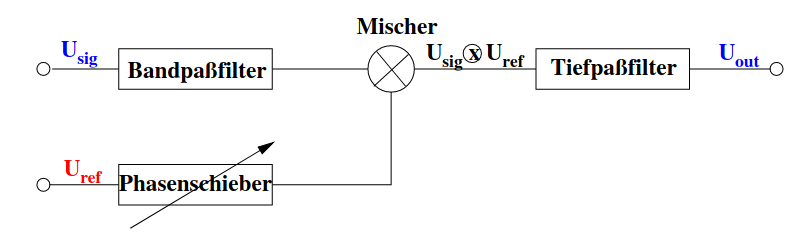
\includegraphics[width=\textwidth]{bilder/schema_lock_in.png}
        \caption{Der grobe schematische Aufbau eines Lock-In-Verstärkers.}
        \label{fig:schema_lock_in}
    \end{figure}

    \noindent In der \autoref{fig:schema_lock_in} ist die grobe Funktionsweise eines Lock-In-Verstärkers zu sehen. Die Signalspannung wird zuert durch einen Bandpass von
    Rauschanteilen höherer ($\omega \gg \omega_{\text{ref}}$) und niedriger Frequenzen ($\omega \ll \omega_{\text{ref}}$) bereinigt. Anschließend wird diese Spannung in 
    einem Mischer mit einer Referenzspannung verstellbarer Phase multipliziert. Die Phasenlage der Referenzspannung ist mit dem Phasenschieber einstellbar. 
    Dann wird das Mischsignal aus Signal- und Referenzspannung durch einen Tiefpass geschickt. Dort wird dieses Mischsignal über mehrere Perioden der Modulationsfrequenz integriert.
    Die Rauschbeiträge, die nicht synchron zur Modulationsfrequenz sind werden so im großteil herausgemittelt. Die Spannung am Ausgang ist eine Gleichspannung, welche 
    proportional zur Eingangsspannung und zum Kosinus der Phasenverschiebung zwischen Signal- und Referenzspannung ist.

    \begin{equation*}
        u-{\text{out}} \propto U_0 \cdot \cos(\phi)
    \end{equation*}

    \noindent Im Gegensatz zu einem Bandpass, welcher Güten von Q $= \num{1000}$ erreicht, kann ein Lock-In-Verstärker Güten von Q$= \num{100000}$ erreichen. Dies liegt an dem 
    Tiefpass, da bei einer großen Zeitkonstante $ \tau = RC$ die Bandbreite des Rauschens $\increment \nu = \frac{1}{\pi RC}$ beliebig klein gewählt werden kann.
    \\
    \\

    \noindent Bei der Betrachtung einer sinusförmigen Signalspannung wird das Vorgehen nun einmal erläutert. 

    \begin{equation*}
        U_{\text{sig}} = U_0 \cdot \sin(\omega t)
    \end{equation*}

    \begin{figure}
        \centering
        \includegraphics[width=\textwidth]{bilder/signalverläufe.png}
        \caption{Die Signalverläufe der verschiedenen Spannungen.}
        \label{fig:signalverläufe}
    \end{figure}

    \noindent In der \autoref{fig:signalverläufe} ist oben die sinusförmige Signalspannung geplottet. Darunter befindet sich die Referenzspannung $U_{\text{ref}}$, welche in diesem 
    Fall eine Rechteckspannung ist, jedoch hat sie die gleiche Frequenz wie die Signalspannung. Die dritte Kurve von oben zeigt das Produkt aus Signal- und Referenzspannung, welches
    im Mischer erzeugt wird. Die letzte aufgetragene Spannung ist die am Ausgang Gemessene, welche wie erwartet eine Gleichspannung zeigt. 

    \noindent Die Rechteckspannung wird durch eine Fourierreihe angenähert. Diese setzt sich aus den ungeraden harmonischen Termen der Grundfrequenz zusammen.

    \begin{equation*}
        U_{\text{ref}} = \frac{4}{\pi} \left( \sin(\omega t) + \frac{1}{3} \sin(3 \omega t ) +  \frac{1}{5} \sin(5 \omega t) + \dots \right) 
    \end{equation*}
    Dann berechnet sich das Produkt aus Signal- und Referenzspannung zu:
    \begin{equation*}
        U_{\text{sig}} \times U_{\text{ref}} = \frac{2}{\pi} U_0 \left(1 - \frac{2}{3} \cos(2 \omega t) - \frac{2}{15} \cos(4 \omega t) - \frac{2}{35} \cos(6 \omega t) + \dots \right) 
    \end{equation*}
    Dieses Produkt besteht aus den geraden Oberwellen der Grundfrequenz $\omega$. Mit dem Tiefpass werden diese Oberwellen dann unterdrückt, dass eine Gleichspannung
    \begin{equation*}
        U_{\text{out}} = \frac{2}{\pi} U_0, 
    \end{equation*}
    die proportional zur Signalspannung ist, herauskommt. In diesem Fall ist $\phi = 0$, welches auch der Fall der maximalen Ausgangsspannung ist, jedoch gilt im Allgemeinen:
    \begin{equation*}
        U_{\text{out}} = \frac{2}{\pi} \cos(\phi)
    \end{equation*}